% !TeX encoding = UTF-8
% !TeX spellcheck = de_DE

%% Dies gibt Warnungen aus, sollten veraltete LaTeX-Befehle verwendet werden
\RequirePackage[l2tabu, orthodox]{nag}

\documentclass[utf8,biblatex]{lni}
\bibliography{che}

%% Schöne Tabellen mittels \toprule, \midrule, \bottomrule
\usepackage{booktabs}

%% Zu Demonstrationszwecken
\usepackage[math]{blindtext}
\usepackage{mwe}

%% BibLaTeX-Sonderkonfiguration,
%% falls man schnell eine existierende Bibliographie wiederverwenden will, aber nicht die .bib-Datei händisch anpassen möchte.
%% Bitte \iffalse und \fi entfernen, dann ist diese Konfiguration aktiviert.

\iffalse
\AtEveryBibitem{%
  \ifentrytype{article}{%
  }{%
    \clearfield{doi}%
    \clearfield{issn}%
    \clearfield{url}%
    \clearfield{urldate}%
  }%
  \ifentrytype{inproceedings}{%
  }{%
    \clearfield{doi}%
    \clearfield{issn}%
    \clearfield{url}%
    \clearfield{urldate}%
  }%
}
\fi

\begin{document}
%%% Mehrere Autoren werden durch \and voneinander getrennt.
%%% Die Fußnote enthält die Adresse sowie eine E-Mail-Adresse.
%%% Das optionale Argument (sofern angegeben) wird für die Kopfzeile verwendet.
\title[Eclipse Che for Education]{Eclipse Che for Fair and Easy Education}
%%%\subtitle{Untertitel / Subtitle} % falls benötigt
\author[Leonhard Applis]
{Leonhard Applis \footnote{Technische Hochschule Georg Simon Ohm, \email{Leonhard.Applis@Protonmail.com}}}
%\startpage{-} % Beginn der Seitenzählung für diesen Beitrag
%\editor{-}    % Namen der Herausgeber
\booktitle{Under Revision for SKILL 2019} % Name des Tagungsband
\year{2019}
%%%\lnidoi{18.18420/provided-by-editor-02} % Falls bekannt
\maketitle

\begin{abstract}
Eclipse Che is a revolutionary cloud-based IDE, inheriting the approach of building cloud-ready software within a 
remote environment. 
Instead of developing on your local machine, a remote development-server is accessed via a webbrowser 
and the artifacts are compiled into docker-containers. 

This paper shortly summarizes the required environment, introduces the concept and workflow of Eclipse Che and evaluates 
the benefits and downsides of this approach. 
Focus is set on a new point of view, enhancing computer studies and 
programming classes with this technology. 
\end{abstract}

\begin{keywords}
Eclipse Che, Cloud-Ready, Cloud-Native, DevOps, Docker, Kubernetes, OpenShift
\end{keywords}

\section{Introduction}
\label{sec:Introduction}
As children we, used to look into the clouds and count sheep. 
As developers, we look into the clouds and check our applications.  
Cloud technologies are already state of the art, enabling global players like Google to run applications on a world-scale.
The market-leaders got their portfolio stocked up with  a  variety  of  different  cloud  technologies,  ranging 
from cloud computing, cloud storage, database-as-a-service or rentable authentication. 
Modern Software needs to be scalable, self-contained, and should run on any device, aswell as in the cloud.  
This trend is also visible in Googles searches \ref{fig:digdocker}. 

\begin{figure}[h]
	\centering
	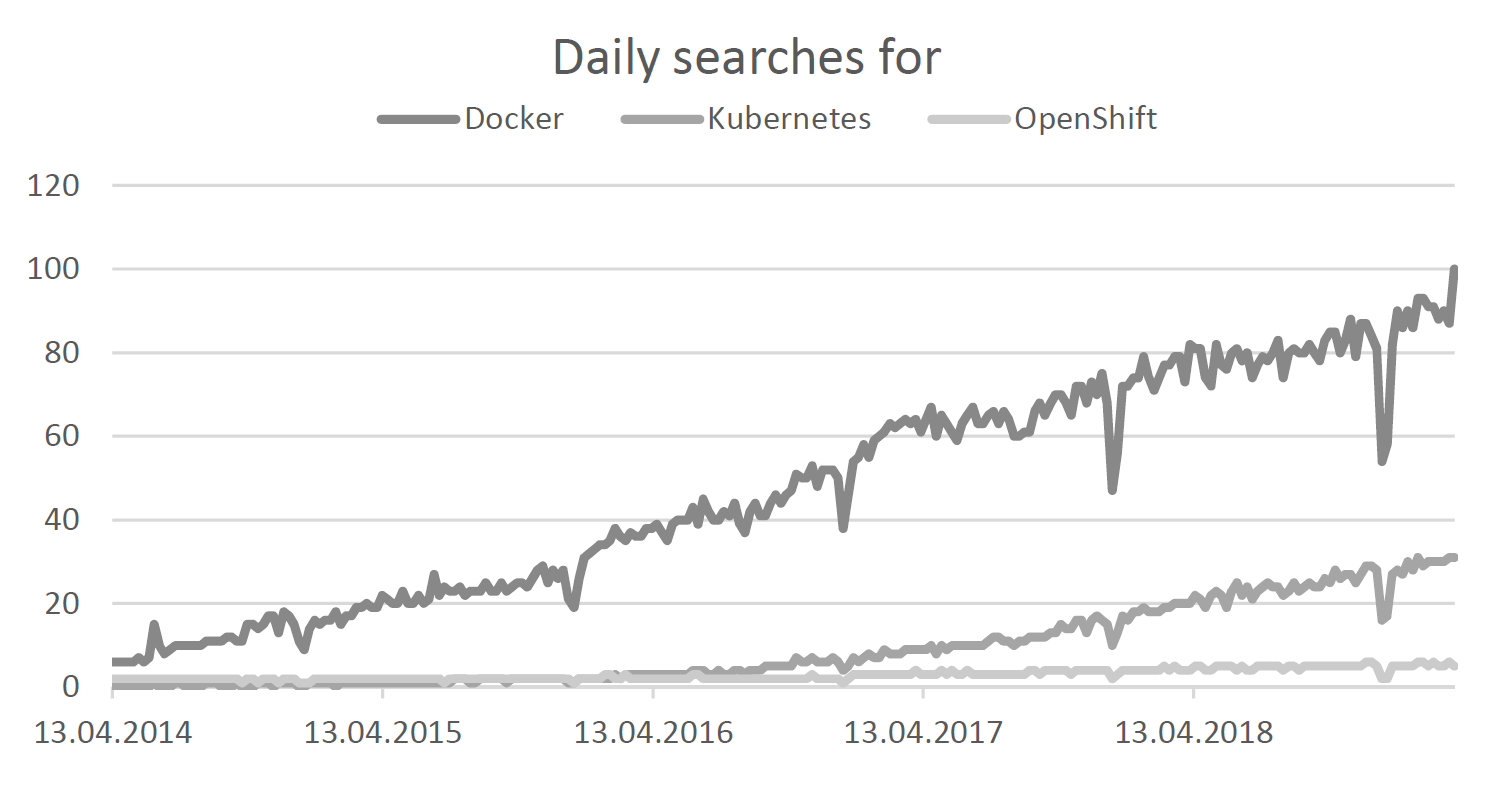
\includegraphics[width=0.5\linewidth]{imgs/DigDocker}
	\caption{Rising interest in Cloud Tec, Data provided by Google Trends}
	\label{fig:digdocker}	
\end{figure}

Figure \ref{fig:digdocker} shows the steadily rising interest in the most popular cloud technologies. 
Docker is a container-engine enabling OS-Virtualization, Kubernetes is a Container-Platform manager and Openshift is a software-suite based on Kubernetes. 
These technologies will be summarized in \ref{subsec:Req}.  
As cloud-technology such technologies are referred which achieve five attributes: 
On-demand self-service, broad network-access, resource pooling, rapid elasticity and measured service [15]. 
Cloud technology usually splits into two components:  Infrastructure  and  Services,  where  docker and Kubernetes are considered infrastructure and provide a  platform  to  host  services.  
Most  of  the  attributes  are (pseudo-) achievable by the infrastructure alone – such as restarting containers. 
Software running as a service can be put into two categories: 
“Cloud-Ready” – meaning that it can be run in common cloud environments, such as Kubernetes. 
The term cloudready  does  usually  not  include  live-scalability. Cloud-readieness is mostly achieved by removing dependencies and either running on bare-linux or being ported into a dockercontainer. 
Lately the term “Cloud-native” came up [17], referring to software which is built from the very first steps to run inside the cloud. This kind of software is usually running inside a docker-container and both resilient and elasticby design [8].  
Resilience refers to the ability of handling failure, both from external sources and restarting/configuring themselves.  
Elasticy is the ability to request more resources on demand, performing more computations when required, but also to free the resources if not needed. 
Cloud-ready Software usually achieves only a certain degree of resilience.   
Cloud-Native applications are aware of their context and collect meaningful metrics for the platform that they cannot reach other services or need more capacities [16]. 
The applications must also be able to use the gained resources in a productive and healthy way.  
Modern  cloud-platforms  can  perform  pseudo-scalabilty for cloud-ready-services by starting multiple instances of the same service. 
The cloud-platform performs load-balancing between these instances. 
This naive approach can work out fine, but for example starting two services working on the same database will not yield any real scalability. 
Another common problem arises when two services are started on the same machine and need the same port, just to name two problems with cloud-ready  software in a cloud environment. 

As Cloud is a central element of modern IT-development, it is strange to see that it is not yet widely teached across 
universities in Germany \footnote{https://www.hochschulkompass.de/studium/studiengangsuche lists currently only 10 german universities with courses on cloud computing, about 30 courses on virtualization }.
There are courses to teach either classic virtualization or docker-basics, but the knowledge of full-stack cloudplatforms and cloud-native development is sealed behind corporate doors and conference workshops.
Meanwhile,  the  annual  Stackoverflow  developersurvey [22] showed, that DevOps-engineers are not only 
amongst the most wanted and most paid jobs but also tend to be the happiest participants.  
Every student either wants to be happy or to be rich, making Cloud an interesting topic for their career. 
So why are there no courses? There are many reasons, but the most prominent is the complexity of the topic: 
To build a real cloud native application, the developer must understand virtualization, system-administration, development, 
infrastructure  and  networking. 
Additionally, the developer needs to use specific tools, know best practices, tests and work in a team.
All these factors make a high stake for entrance, also  represented in the developersurvey [22] which states that most DevOps engineers have a decade of experience, usually in operations topics.
Lucky for us, a new open-source software, Eclipse Che, is on the rise to enable everyone for cloud-native development.
Che is unlike a normal eclipse distribution: 
It is hosted on a server and developers get access with their browser. 
Instead of installing dependencies, compilers etc. locally, a common workspace is set up, which is shared amongst the programmers. 
The software build is run inside a docker-container, making it cloud-native by default. 
With Version 7 upcoming and prominent support from RedHat, Eclipse Che is not a prototype anymore. 
The latest distributions of RedHats OpenShift are shipped with Che in default. 
Therefore, it is worth looking at this possible game-changer. 
With the first part of this paper, the structure and ideas of Che are explained in more detail, the second part of this pa-
per covers general arguments about this approach and gives a detailed overview of reachable benefits for education.    

\section{Eclipse Che}
\label{sec:Che}
\subsection{Environment and Requirements}
\label{subsec:Req}
Che is hosted as a server-application and is already cloudnative. 
The only requirements are that either Docker, Kubernetes or OpenShift are available for the installation.
The differences between these will shortly be summarized.
 
Docker\footnote{https://www.docker.com/} is a container-plattform, where a container is a standardized unit of of software including the code, dependencies and core-functionalities. 
A container runs on an OS-Virtualization, originating from LXC, has declared interfaces and can be parameterized. 
One of the core features is to connect containers for bigger projects, e.g. one 
database container and one web-server container, which are connected into a virtual network. 
Docker is mostly famous for this docker-engine, but enriches it with monitoring and logging, as well as the ability to move containers onto different machines.   

Kubernetes\footnote{https://kubernetes.io/} is a container-orchestration-system based on Docker. 
Kubernetes picked up the growing problem in managing multiple docker-containers by  simplyfing  resource-management. 
Additional to deployment and monitoring of container-groups it provides auto-restart mechanisms and scaling based on (custom) metrics. 
When run on Kubernetes, Che is hosted as a single docker container in the existing platform.
The term pod, also later used in this paper, refers to a suite of connected containers. 
An example pod would be a simple two-tier web-application, where the database and webserver are two different, but connected containers.

Openshift\footnote{https://www.openshift.com/} provides a software-suite around Kubernetes with the goal to automate cloud-native development and delivery.
Notable  additions  include  Jenkins,  Gitea,  Sonarqube and lately Che. 
Regarding Che there are no notable changes in handling, as Che is simply run on the build in Kubernetes.
When run on Kubernetes or Docker Che will require two additional containers for authentification with KeyCloack. 
For Openshift the standard-openshift authentification is used.  
Eclipse Che  can be run  on any  base-technology  on  localhost – this is rather for demonstrations aswell as for developers working on the Che-Code. 
When run (locally) on docker, the plugin CheDir enables a portable workspace, 
which can be used on any docker based Che.
\subsection{Technology and Workflow}
\label{subsec:Tec}
A normal IDE is software on your computer which makes programming easier than doing it in a plain text-editor and commandline. 
Common tasks for an IDE are dependency management, debugging, refactoring and autocompletion.
It is important that an IDE is not required to develop – you can write .java-files in Vim, compile on the console and run a .Jar manually. 
With that in mind, we can see that the IDE is just a tool to make things (a lot) more comfortable – but you also have requirements such as the JDK, the .Jars you need in your classpath etc. as they are only utilized by your IDE.
You can consider this stack as your workspace as it contains everything required to work, with the IDE making the workspace comfortable to use.
Eclipse Che does not work like a normal IDE. 
Che consists of three main components shown in Figure \ref{fig:cheworkflow}\footnote{source:\url{https://en.wikipedia.org/wiki/Eclipse_Che#/media/File:Eclipse_Che_-_Workflow.PNG}}.

\begin{figure}[h]
	\centering
	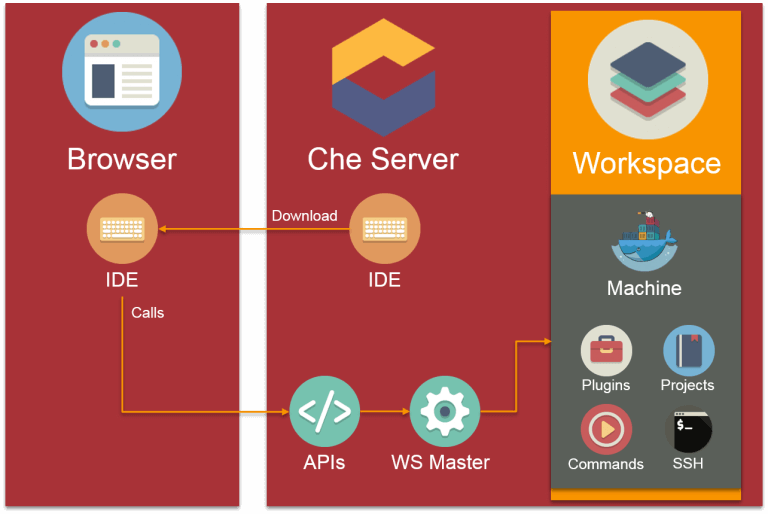
\includegraphics[width=0.7\linewidth]{imgs/Che_Workflow}
	\caption[Che Workflow]{Che Workflow}
	\label{fig:cheworkflow}
\end{figure}


\begin{enumerate}
	\item Workspaces, including Runtimes and IDEs
	\item A browser-based IDE
	\item An administrative server
\end{enumerate}
A workspace is like your above mentioned common \textit{workspace}. 
It is a single machine, as a container, containing the project files, compilers, package managers and an IDE-Interface. 
There are two big differences to a normal development-setup:
\begin{itemize}
	\item The required items for the workspace are explicitly  declared, making  the  workspace itself a docker image
	\item The IDE is not graphical – it is a REST-API performing actions like a normal IDE, such as build, writing to files and installing packages.  
\end{itemize}
An additional distinction is about building your software.
Instead of building the .Jar in your remote-workspace, it is build inside a container in the remote-workspace.
While this sounds a bit confusing, it makes sense to separate the actual runtime from the workspace. 
This is also what happens on your machine – you compile an executable and run it separately. 
Having these runtimes inside a docker-container comes with great benefits, outlined later in this paper.
The second component is the web-based IDE, which is basically a webpage performing the required REST-calls and utility-tasks for the developer. 
It is sent by the administrative server when an authorized user accesses his workspace via browser. 
These two components can be enriched with plugins.  
Common plugins are language-extensions which support syntax-highlighting etc. or package managers with their regarding lifecycles.
The difference to a normal IDE plugin is that it has two components: 
One in the workspace-API and one in the hosted web-IDE.  
Che offers a suite of common plugins dependent on your project. 
When starting a Maven-project, the workspace is initialized with Maven and Java.
The last component is the Che-administration server. 
In the administration-server the workspaces are orchestrated and monitored. 
The authorization is also done at the admin-server and not by every workspace.
The workspaces can be split amongst multiple machines.
The runtimes do not necessarily need to be on the same machines as their workspaces. 
Instead of the web-based IDE, you can connect a desktop IDE to your workspace. 
This is done by mounting the workspaces-filesystem  in  your  desktop  IDE. 
This  will grant you access to autocompletion and other features, but you will miss Che specific helpers the web-IDE offers. 
My personal oppinion is, that mounting remote file systems for development sounds like a infinite source of problems. 
I expect this feature to be rather a proof of concept.
A single workspace can contain multiple projects, whereof every project will have its own runtime. 
Projects can either share a versioning control or be separated. 
You can build whole pods in a single workspace with the single containers being the subprojects. 
You can also compose applications inside the workspaces, meaning that the resulting 
container of a project can be the base-image of another project. 
A workspace can be shared amongst multiple users. 
Both will work on the same remote filesystem, altering files simultaneous. 
Due to changes being transmitted as HTTP-requests, the current implementation when working on the same file is a \textit{last write wins}-policy. 
For version 7 a multi-cursor file-editing will be provided, like it`s common in 
drive-documents. 
This is not to be mixed up with having multiple users work on the same project but on their own workspaces. 
The code, and the workspace itself, can commonly be shared with any versioning tool like Git.
It's mostly dependent on the team which kind of cooperation they prefer. 
As  an  interesting  fact,  Eclipse  Che  is  developed  with Eclipse Che, proving that complex cloud development is possible. 
This so-called \textit{dogfooding} usually leads to a product which puts requirements over any a-priori design or foreign interests.  
Existing components will be enhanced if working with them becomes troublesome, leaving a clean and valuable core product. 

\section{General Benefits and Handicaps}
\label{sec:Eval}
The primary goals of Che are twofold: 
First it reduces failure when migrating software into the cloud and enhances the experience of working in a rich remote environment.
Second is to set up people into existing projects faster and failsafe.

The university of Arizona showed [11], that about 50\% of software inspected was not able to build. 
Common reasons are missing, changed or faulty dependencies, leading to the common term of \textit{dependency hell} aswell as unclear documentation. 
Experienced programmers are usually able to overcome these issues, given enough time. This continues to be an issue [14], and without a different approach probably always will be. 
This problem is solved, if the software is built inside a docker-container and follows the principles of self-containment and image-immutability [17].
The self-containment principle dictates that  at build-time every required dependency is given, and a fully functional image is created.
A dockerized maven-application would include java, maven and every required maven package to run the application in the current state. 
The image-immutability means to forbid alternations to the environment. 
No installations at runtime, no change in ports, no creation of database-schemas.
These two principles, while being optional, lead to always reproducible and functional artifacts.
The main challenge is to migrate existing software and fulfill these properties. 
Typically, after making the first iterations of your software on your local machine, dockering it will yield to 100 problems at once, not only being frustrating but taking tons of time. 
With Che, this kind of Big-Bang-Migration is not possible, as from the very first step you are working inside of a docker-container.
The properties above can be hold with every change to the image and checked in a normal review-process. 
Problems will arise one at a time and be solved one at a time, whether they are about code or operations. 
Che therefore embraces the core-ideas of DevOps [19][20] and agile software development [18].
That being said, of course it's possible to big-bang-migrate into Che, causing the normal problem mentioned above. 
However, once the errors are resolved, every further development will work more agile by design.
The artifacts (whether containers or pods) produced with Che are self-contained and immutable, therefore every result is reproducible. 
Any further development is incremental on the existing images and keeps old artifacts stable. 
As the code is fully build inside containers and are already run remotely, the famous “It works on my Machine!” is eliminated. 
This does not only enhance deployments, but also has a big impact on quality assurance and the motivation of developers. 
You can keep multiple projects in a single workspace and launch multiple pods at once, running the full environment. 
The behavior of this multipod is unified and testable, making a stable release of full environments possible. 
This is one of the primary goals of the DevOps approach [20]. 
The workspace can therefore form totally new ways of programming, such as IoT Applications \footnote{he Plugin Arktik for Eclipse offered IoT Development with Che.While Arktik is unsupported since February 2019, it proved that the concept worked.} or a full setup of microservices [21], while being agile and reproducible.
Onboarding new teammembers is made easy with Che. 
A newly joining member does not need to install IDEs, languages, tools and packages, he only needs access to his Che-Account and a singular workspace with every dependency build for him.
Depending on the complexitiy of the project this required atmost an hour. 
While this may seem long, the setup time is dependent on the complexity of the workspace. 
Setting up a complex workplace will also take more time manually. 
The work for this is done automatic and remote, so the user is free to dive into the documentation or have some coffee. 
His workspace will be able to launch the latest version immidieatly.
It is also notable, that the (technical) onboarding of developers and operators is streamlined into one single process. 
The combination of a quick setup and the usability of every enhancement makes Che especially interesting to recruit troubleshooters into your projects, which solve some of the very specialiced tasks.  
With  the  artifacts  being  reproducible,  the  expert  can quickly inspect the subject and analyse problems.
With a finished workspace he can quickly start working. 
With his changes being also in docker, they will be visible and functional for the whole team.
Therefore,  the  hardest  common  problems  regarding \textit{quick help} are addressed and solved. 
As an additional minor benefit, it is easy to hibernate resources  using  Che  with  Kubernetes  or  Openshift.
The workspaces collect metrics like any other container and are therefore scalable on demand. 
The ability of downscaling the development resources has a big impact on the overall 
workload. 
As a further example, the workspaces could be shut down out of normal business-time. This attribute is crucial for a rented infrastructure, which is paid commonly on both workload and storage.  
The very first handicap coming with Che is the requirement for a good internet connection. 
While your normal buro is already equipped with internet, one may want to work on train or there is simply a problem with the WiFi in your hotel.
With the possibility to setup che on localhost, you can learn the basics and routines offline. 
As the main benefits come in terms of teamwork, this is not a real solution.
The primary problem with Che is the requirement for an already dense knowledge of cloud related technology.
Setting up the Workspace, docker-images, build and CI scripts is a complex topic and can not be done by someone getting started. 
This requirement extends when working with a multipod-environment. 
While most of the tasks are by themselves rather simple, the bare amount of such tasks (especially when migrating an existing project to Che) requires a broad knowledge.
This can be done by a single expert user, enabling the other developers  to  use  the  build-routines and  environments provided. 
However, many problems which arise are related to the cloud-environement and will be hard to solve by a novice user, making him dependent on the expert. 
It's therefore necessary to get everyone on a certain base-level to solve their own problems, otherwise the expert will be overloaded and the project stuck.  
Additionally, the missing default “build and run” is a paradigm-shift for many developers, which will take a while to get used to. 
Clark et al. [14] describe this rather as a change in the mindset, than in actual technology: 

TODO CITE CITE CITE
The primary shift that’s required is not one of new tooling, as most developers already have the basic tooling they need. 
Rather, the needed shift is one of philosophy. 
TODO CITE CITE CITE END

Intuitively this is true: Every developer needs to setup his own workspace – the skills to do this are already there. 
The only difference is to setup the workspace in a common, documentated and descriptive way. 

Another problem with Che is the uncommon debugging. 
As the code is running in a remote-runtime, the common breakpoint  and  valuecheck
is  missing.  
Instead,  one  either must be familiar with the languages commandline-debugging or write good logs and metrics. 
While this will slow down development, it also offers some benefits: 
The debugging and error-analysis inside the container is the same as it would be in the productive environment. 
Having meaningful logs with different loglevels and collecting valuable metrics is 
in general a good attribute for software in any circumstance. 
It just means additional effort and know-how.  
The last problem is the vulnerability to malevolent users. 
Someone who already is in possession of a valid account can drain the shared resources of a full cluster, therefore blocking  any  other  user  from  work.
This  can  also  be achieved by human error. 
Dependent on the setup, the attacker could also auto-deploy hidden spyware into a pro-
duction environment. 
While this is also a problem for normal developer teams, the fast pace of deployments with Che requires additional care. 
A rich CI/CD environment, such as a well-maintained Jenkins may lead to less-detailed code-reviews, as both unit- and end-to-end-tests succeed.  
It is therefore important to not only restrict access to project resources, but also the double-check and guard the releases.  
Some security risks can also emerge from docker-images as well [9] but are out of scope for this paper.

\section{Benefits for Education}
\label{sec:EvalEdu}
In addition to the previous mentioned benefits, there are more points about Che that are especially important for educational purposes, such as courses in the university, professional school or research departments.
For simplicity I will only elaborate universities, to which I can best relate.
Eclipse Che provides the possibility to learn primary cloud-technologies hands on and in a simple and supportive manner. 
Unfortunetally, these topics are currently not widely teached at university.
Che makes it possible to teach students fundamentals of modern software development.
Depending on the courses subject, one can either provide scalable software or a running environment. 
With fitting material provided, it's easy to learn cloud-native development, DevOps or Cloud-Operations. 
Even complicated topics, like microservices and IoT-applications can easily be adaptet inside Che [21] and performed as for example as group-projects with a common goal. 
The student will need to understand cloud-components aswell as team-work to succeed with Che. 
The produced artifacts can simply be shipped as containers, giving comfortable access to the professor. 
With both the product and the code inside the workspace easily accessible, the professor can grant faster and better feedback for the students, which can have massive impact on learning [1][5].
Additionally, the professor can provide automated end-to-end tests with tools like Jenkins or TravisCI. 
Given such an environment, the student will immideatly get objective feedback, whether their code fulfills the requirements. 
This immediate feedback is a big motivator and has a positive impact on the learning experience [2]. 
With a clear reason on the usefulness of the task, the visible progress and the direct impact of personal effort should lead to intrinsic motivation, which studies show to have a strong effect on education [23]. 
As a requirement, it's necessary to provide a meaningful and fun task. 
Fortunately, such tasks are not that rare in development.  
Other studies have shown that only automated and unified testing is not beneficial to education in general [3]. 
But the tools provided by Che and CI/CD slim down the overhead until both personal feedback and automated can be supplied. 
If the whole classroom utilizes this system, the educator can also monitor who is having trouble in an automated manner. 
With a single investment for the tests, feedback for every student is granted at every time. 
With the single investment of providing a running Che instance (and a short lecture how to use it), feedback on the artifacts and code can be immidieatly granted to every student, without having the overhead of setting up workspaces. 
These investments can be done before the course starts at any time and can be reused.
It's not dependent on the individual students. 
In general, this approach enables studies to be less about the subject, but instead to be about learning the subject. 
I consider this the primary goal of university courses. 
Another benefit for education is about fairness in IT-Education.  
With access to a university Che workspace, every person can develop the same software in the same environment. 
A wellknown problem is the necessity of an IOS-build-device for IOS-appdevelopment.
Students which are limited in their access to the university-laboratory or cannot afford a mac are therefore handicapped.
Another  rising  problem  are  GPU-accelerated  machine learning algorithms. 
Depending on the task, training neural networks can be 20 times faster if a CUDA-compatible graphics card is used. 
The range for these graphiccards start at 300\$ and are therefore not commodity hardware,especially for students.  
While these technologies are great and important for many applications, the required technologies are exclusive due to  their  costs.
This  hindrance  for  education  is  usually adressed  with  IOS-laboratories  and/or  cloud-resources paid for by university. 
The topic of socio-economic factors is beyond the scope of this work, but the impact has been analyzed by the PISA Studies [7], which state that socio-economicly handicapped students fail three times more likely to achieve a basic level of performance.
According to PISA, this rate has not significally changed since the studies started in 2006. 
Germany scored on the impact of socioeconomic-factors on education better than it did in 2006 but is worse than global average [6].
The Mac-Laboratories and rented cloudspace are technically a good attempt at inclusion. 
But students which are required to get to university to do their assignments are 
less  likely  to  do  so.
Making  assignments  mandatory, providing extrinsic motivation [23] has usually a negative impact on the subjective experience.
A different problem comes with machine-learning, which is usually a process of trial and error to some extend.
Long waiting times disconnect the action from the result being not beneficial for the learning process [1][23]. 
One may argue that having this kind of anticipation is extra rewarding and therefore highly motivational.
From my personal experience, working in this modus becomes exhausting after a period of weeks, especially when errors occur. 
I expect this experience to be highly personal. 
I think providing the fastest infrastructure possible, enabling the fastest results, is the better way. 
Making progress slower is much easier than making it faster.  
In addition, the time spent waiting on your machine learning algorithm or moving to the mac-laboratory on weekends is simply dead time. 
It should therefore be minimized.   
With studies showing basics of good learning experiences [2][3] and the impact of motivation [1][23], it is mandatory for institutions to provide the best possible environment. 
While many socio-economic factors cannot be grasped at the university or by the educators, those originating in the students' economic background can be addressed.
Most universities already provide free services, such as software-suites, e-libraries or cloud storage.
Simply providing a technical correct solution (like laboratories) is not enough to provide a good environment.
One student with a better socio-economic background who can afford a 300\$ GPU will have a better baseline for his education. 
This is simply put unfair.
With Che, universities can provide a free, good and accessible development environment for every student.
\section{Conclusion}
\label{sec:Conclusion}
Cloud technology will be dominant in the foreseeable future. 
Not \textit{everything} will be best fit for cloud, but most of the everyday software benefits from the concepts. 
With more and more tools making it easier, it's just a matter of time until cloud-tec becomes standard instead of bonus.
With Eclipse Che many problems about teaching students these Cloud Skills and reducing the initial scope for learning, are addressed. 
While the impacts on motivation and the actual learning results are only hypothetical, most of the technical aspects are solved by Che.  
As Eclipse Che is cutting edge it whatsoever lacks many quality of life features, has some bugs, and the design is undefined to some extend. 
It somewhat is a chance: 
Instances like a university can have massive impact on the design of Che and drive the project to some extend for their own needs. 
With faculties working on the open source project, either providing code and features, or just testing Che in educational environments, both quality issues and missing features can be solved.    
Now cloud development is only for corporations. 
There is hardly any chance to successfully learn it at university. 
With Che there is another chance to “get back into the game” – and provide corporation-free education.  
While this sounds harsh towards companies, I think unbiased education for students is not a nice thing to have, but a core concept of education in general. 
Only if that is true, the students can make unbiased decisions and make unbiased research. 
Being dependent on Google for Universities is in a similar way disturbing, as if a biology faculty would be sponsored by Bayer. 
One can only imagine a grim future if the curriculum is influenced by profit. 
\section*{Future Work}
\label{sec:FutureWork}
As this paper only summarizes benefits and outlines some ideas, the next step would be to put it to the test.
In addition, a study could be elaborated on both the acceptance and effect of a CI/CD based development course with Che. 
Unfortunately, the study would lack any comparison as there are few courses on this topic. 
These studies could be done with universities and corporations, which 
may yield very different results.   

%% \bibliography{lni-paper-example-de.tex} ist hier nicht erlaubt: biblatex erwartet dies bei der Preambel
%% Starten Sie "biber paper", um eine Biliographie zu erzeugen.
\printbibliography

\end{document}
